%@AUTHOR: Cardel
%Configuracion del documento

\documentclass{beamer}
\usetheme{Berkeley}
\setbeamertemplate{caption}[numbered]
\usepackage{graphicx}
\usepackage[utf8]{inputenc}
\usepackage[spanish]{babel}
\usepackage{ragged2e}
\usepackage{colortbl}
\usepackage{color}
\definecolor{naranja}{rgb}{1,0.5,0} % valores de las componentes roja, verde y azul (RGB)
\definecolor{rojo}{rgb}{1,0,0}
\definecolor{SteelBlue}{rgb}{0.3,0.5,0.7}
\usepackage{float}

\author{Carlos Andr\'es Delgado S.} 
\title{710193M Arquitectura de computadores II}
\subtitle{Repertorio de Instrucciones \\ carlos.andres.delgado@correounivalle.edu.co}
\institute{Facultad de Ingeniería. Universidad del Valle}
%Transparencia
\setbeamercovered{transparent}

%LOGO Univalle
\pgfdeclareimage[height=1.4cm]{logo}{imagenes/univalle}
\logo{\pgfuseimage{logo}}

\usepackage{listings}% http://ctan.org/pkg/listings
\usepackage{listingsutf8}

\lstset{ %
  basicstyle=\footnotesize,           % the size of the fonts that are used for the code
  numbers=none,
  numberstyle=\footnotesize,          % the size of the fonts that are used for the line-numbers
  numbersep=4pt,                  % how far the line-numbers are from the code
  backgroundcolor=\color{white},      % choose the background color. You must add \usepackage{color}
  breaklines=true,                % sets automatic line breaking
  breakatwhitespace=true,        % sets if automatic breaks should only happen at whitespace
  title=\lstname,                   % show the filename of files included with \lstinputlisting;{}
  extendedchars=false,
  inputencoding=utf8, 
  tabsize=2,
   mathescape=true,
  literate={\ \ }{{\ }}1
}
\newsavebox{\myLst}
\newsavebox{\myLstb}
\newsavebox{\myLstc}
\newsavebox{\myLstd}

\usepackage{enumitem} % enumerados

%Para que en cada seccion aparezca la tabla de contenido
\AtBeginSection[]{
	\begin{frame}
	\frametitle{Contenido}
	\tableofcontents[currentsection]
\end{frame}
}

\AtBeginSubsection[]{
	\begin{frame}
	\frametitle{Contenido}
	\tableofcontents[currentsubsection]
\end{frame}
}



\date{Marzo de 2016}
\newcommand{\grad}{\hspace{-2mm}$\phantom{a}^{\circ}$}
\begin{document}

\begin{frame}
	\titlepage	 		
\end{frame}

\begin{frame}
	\tableofcontents	 		
\end{frame}


\section{Características y funciones}

\begin{frame}
	\frametitle{Instrucciones}
	\begin{block}{Que es una instrucción}
	\begin{enumerate}
		\item Instrucciones comprendidas por el computador
		\item Código de máquina
		\item Son binarias
		\item Se representan por códigos de ensamblador (ADD, MV, etc)
	\end{enumerate}
	
	\end{block}		 		
\end{frame}

\begin{frame}
	\frametitle{Instrucciones}
	\begin{block}{Elementos esenciales instrucción}
	\begin{enumerate}
		\item Código de operación
		\item Referencia a operandos fuente y destino
		\item Referencia a la siguiente instrucción
	\end{enumerate}
	
	\end{block}		 		
\end{frame}

\begin{frame}
	\frametitle{Instrucciones}
	\begin{block}{Código de operación}
	Especifica el tipo de operación a realizar:	
	\begin{enumerate}
		\item Aritméticas o lógicas
		\item Transferencia de datos entre dos registros
		\item Transferencia de datos entre dos registros y memoria
		\item Transferencia de datos entre dos posiciones de memoria
		\item Captación y envío de datos de dispositivos E/S
		\item Control
	\end{enumerate}	
	\end{block}		 		
\end{frame}

\begin{frame}
	\frametitle{Instrucciones}
	\begin{block}{Referencia a operandos}
	Especifican posiciones memoria o registros, los datos pueden ser direcciones, números, caracteres o datos lógicos.
	\end{block}	
	\begin{block}{Referencia a la siguiente instrucción}
	Está implícita en la instrucción.
	\end{block}		 		
\end{frame}

\begin{frame}
	\frametitle{Instrucciones}
	\begin{figure}[H]
	\centering
	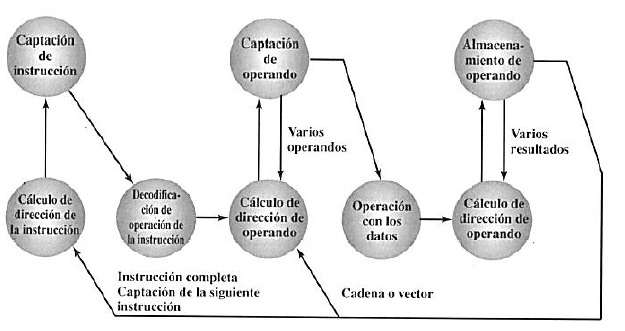
\includegraphics[scale=0.35]{imagenes/instruccionmaquina.jpg}
	\caption{Instrucción de máquina}
	\end{figure}
	
	\begin{block}{Elementos instrucción}
	\begin{itemize}
		\item El funcionamiento de la CPU está determinado por las instrucciones que ejecuta
		\item Al conjunto de instrucciones se le denomina \textbf{repertorio de instrucciones}
	\end{itemize}
	\end{block}		 		
\end{frame}

\begin{frame}
	\frametitle{Instrucciones}
	\begin{block}{Elementos instrucción}
	\begin{itemize}
		\item \textbf{Código de operación:} Especifica la operación a realizar
		\item \textbf{Referencia a operandos fuente:} Los operandos de entrada a la instrucción
		\item \textbf{Referencia al operando resultado:} La operación puede producir un resultado
		\item \textbf{Referencia a la siguiente instrucción:} ¿Donde está la siguiente instrucción?. Se define por el contador de programa (PC)
	\end{itemize}
	\end{block}		 		
\end{frame}


\begin{frame}
	\frametitle{Instrucciones}
	\begin{figure}[H]
	\centering
	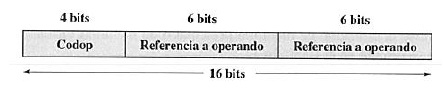
\includegraphics[scale=0.8]{imagenes/formatoinstruccion.jpg}
	\caption{Instrucción de máquina}
	\end{figure}
	\begin{block}{Formato de instrucción}
		\begin{itemize}
			\item Se representa por una secuencia de bits
			\item Durante su ejecución, la instrucción se escribe en un registro de instrucción (IR)
			\item La CPU debe extraer los datos de los distintos campos de la instrucción para realizar la operación
		\end{itemize}
	\end{block}		 		
\end{frame}


\begin{frame}
	\frametitle{Instrucciones}
	\begin{block}{Representación de instrucciones}
	Debido a la complejidad de manejar instrucciones en binario, se utilizan representaciones simbólicas llamadas \textbf{Nemotecnicos}
		\begin{itemize}
			\item \textbf{ADD:} Sumar
			\item \textbf{SUB:} Restar
			\item \textbf{MPY:} Muliplicar
			\item \textbf{DIV:} Dividir
			\item \textbf{LOAD:} Cargar datos en memoria
			\item \textbf{STOR:} Almacenar datos en memoria
		\end{itemize}
	\end{block}		 		
\end{frame}

\begin{frame}
	\frametitle{Instrucciones}
	\begin{block}{Representación de instrucciones}
		\begin{itemize}
			\item Un lenguaje de alto nivel (C, C++, Java, etc) representa las operaciones utilizando variables
			\item Un lenguaje de máquina expresa las operaciones de una manera elemental, implicando operaciones de transferencia de datos, entre otras.
			\item \textbf{Cualquier programa escrito en un lenguaje de alto nivel, debe traducirse a lenguaje de máquina}
		\end{itemize}
	\end{block}		 		
\end{frame}


\begin{frame}
		\frametitle{Instrucciones}
		\begin{block}{Representación de instrucciones}
		\begin{itemize}
			\item Un lenguaje de alto nivel (C, C++, Java, etc) representa las operaciones utilizando variables
			\item Un lenguaje de máquina expresa las operaciones de una manera elemental, implicando operaciones de transferencia de datos, entre otras.
			\item \textbf{Cualquier programa escrito en un lenguaje de alto nivel, debe traducirse a lenguaje de máquina}
		\end{itemize}
	\end{block}		 		
\end{frame}

\begin{frame}
		\frametitle{Instrucciones}
		\begin{block}{Clasificación de instrucciones}
		\begin{itemize}
			\item \textbf{Procesamiento de datos:} Pueden operar datos aritméticos o lógicos
			\item \textbf{Almacenamiento de datos:} Instrucciones de memoria
			\item \textbf{Transferencia de datos:} Instrucciones a dispositivos E/S (Teclado y monitor principalmente)
			\item \textbf{Control} Instrucciones de comprobación (Comprobación de zero, negativo).			
		\end{itemize}
	\end{block}		 		
\end{frame}


\begin{frame}[fragile]
		\frametitle{Instrucciones}
		\begin{block}{Número de direcciones}
		\begin{itemize}
			\item \textbf{3 direcciones:} Dos operandos y un resultado $ a = b + c$
			\item \textbf{2 direcciones:} Un operando y un resultado: $a = a + b$
			\item \textbf{1 dirección:} Un operando, utiliza un acumulador para almacenar los resultados.
			\item \textbf{0 direcciones:} Las direcciones son implicita,s, ejemplo push a, push b, etc.
		\end{itemize}
	\end{block}		 		
\end{frame}



\begin{frame}
		\frametitle{Instrucciones}
		\begin{block}{Diseño del repertorio de instrucciones}
		\begin{itemize}
			\item Es complejo, ya que afecta las funciones dela CPU
			\item Es el medio que tiene el programador de controlar la CPU
			\item \textbf{Repertorio de instrucciones:} Cuantas operaciones se tienen
			\item \textbf{Tipos de datos:} Que datos son utilizados en las operaciones: numéricos, boleanos, texto, etc.	
		\end{itemize}
	\end{block}		 		
\end{frame}


\begin{frame}
		\frametitle{Instrucciones}
		\begin{block}{Diseño del repertorio de instrucciones}
		\begin{itemize}
			\item \textbf{Formato de instrucciones:} Longitud de la instrucción (en bis), número de direcciones, tamaño de los campos.
			\item \textbf{Registros:} Número de registros de la CPU que pueden ser referenciados
			\item \textbf{Direccionamiento:} Modo o modos de direccionamiento mediante los cuales puede especificarse la dirección de un operando	
		\end{itemize}
	\end{block}		 		
\end{frame}



\section{Modos de direccionamiento}

\begin{frame}
		\frametitle{Modos de direccionamiento}
		\begin{block}{Tipos de direccionamiento}
		\begin{itemize}
			\item \textbf{Direccionamiento inmediato:} Se envía el dato directamente
			\item \textbf{Direccionamiento directo:} La dirección del operando está en el campo de direcciones
			\item \textbf{Direccionamiento de indirecto:} El campo de direcciones apunta a la posición que contiene la dirección del operando
			\item \textbf{Direccionamiento a registro} Puede ser directo, indirecto o con desplazamiento	
		\end{itemize}
	\end{block}		 		
\end{frame}


\begin{frame}
	\frametitle{Modos de direccionamiento}
	\begin{block}{Direccionamiento inmediato}
		El operando está presente en la instrucción:
		\begin{equation}
			Operando = A
		\end{equation}
		Donde $A$ es una constante que puede ser numérica, booleana, carácter, etc. Ejemplo $ADD 5$.				
	\end{block}		 		
\end{frame}

\begin{frame}
	\frametitle{Modos de direccionamiento}
	\begin{block}{Direccionamiento inmediato}
	\frametitle{Instrucciones}
	\begin{figure}[H]
	\centering
	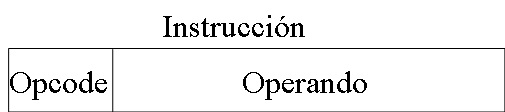
\includegraphics[scale=0.4]{imagenes/inmediato.jpg}
	\caption{Direccionamiento inmediato}
	\end{figure}			
	\end{block}		 		
\end{frame}

\begin{frame}
	\frametitle{Modos de direccionamiento}
	\begin{block}{Direccionamiento directo}
		El operando contiene la dirección efectiva del dato
		\begin{equation}
			EA = A
		\end{equation}
		Donde $EA$ es la dirección del dato $A$. Ejemplo $ADD [2]$, donde $[2]$ es la dirección que contiene el dato .				
	\end{block}		 		
\end{frame}

\begin{frame}
	\frametitle{Modos de direccionamiento}
	\begin{block}{Direccionamiento directo}
	\begin{figure}[H]
	\centering
	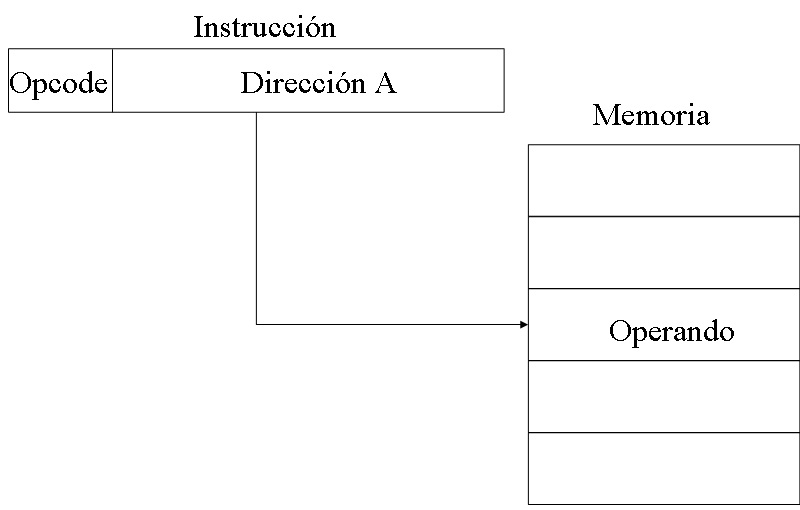
\includegraphics[scale=0.4]{imagenes/directo.jpg}
	\caption{Direccionamiento directo}
	\end{figure}			
	\end{block}		 		
\end{frame}

\begin{frame}
	\frametitle{Modos de direccionamiento}
	\begin{block}{Direccionamiento indirecto} \justify
		El problema del direccionamiento directo es la longitud del campo de direcciones que normalmente es menor que la longitud de la palabra, limitando el rango de direcciones. Una solución es que el campo de direcciones referencie a la dirección a una dirección en memoria
		\begin{equation}
			EA = (A)
		\end{equation}
		Donde $EA$ es la dirección del dato $(A)$ el cual contiene la dirección al dato. Ejemplo $ADD ([2])$, donde $([2])$ es una dirección a una localización de memoria que contiene la dirección del dato del operando.				
	\end{block}		 		
\end{frame}

\begin{frame}
	\frametitle{Modos de direccionamiento}
	\begin{block}{Direccionamiento indirecto}
	\frametitle{Instrucciones}
	\begin{figure}[H]
	\centering
	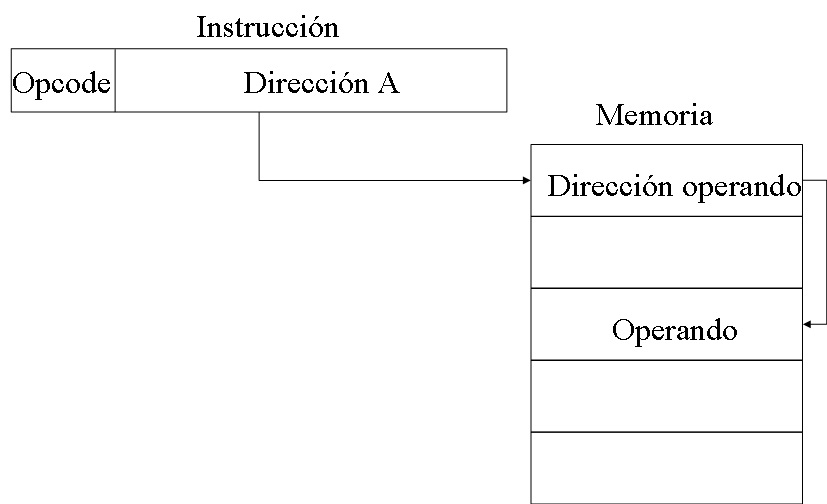
\includegraphics[scale=0.4]{imagenes/indirecto.jpg}
	\caption{Direccionamiento directo}
	\end{figure}			
	\end{block}		 		
\end{frame}

\begin{frame}
	\frametitle{Modos de direccionamiento}
	\begin{block}{Direccionamiento directo con registro}
		El registro contiene la dirección efectiva del dato
		\begin{equation}
			EA = R
		\end{equation}
		Donde $EA$ es la dirección contenida en el registro $R$. Ejemplo $ADD [X]$, donde $[X]$ es el registro que contiene el dato.				
	\end{block}		 		
\end{frame}

\begin{frame}
	\frametitle{Modos de direccionamiento}
	\begin{block}{Direccionamiento directo con registro}
	\begin{figure}[H]
	\centering
	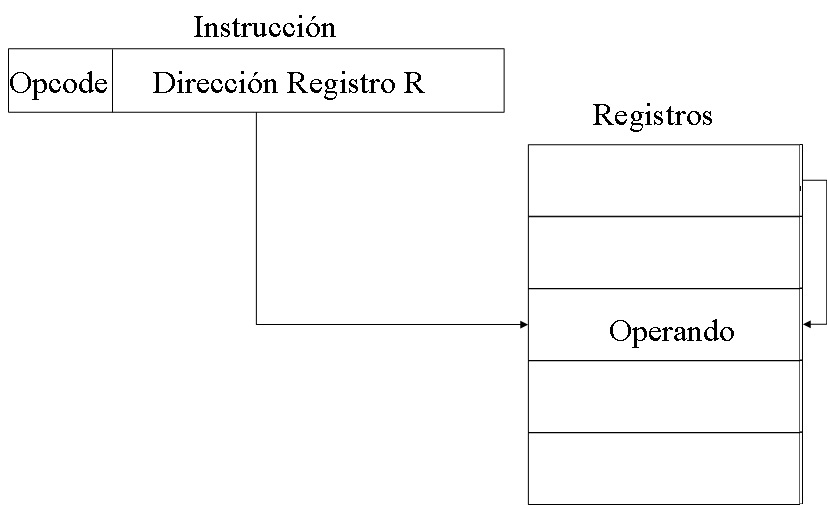
\includegraphics[scale=0.4]{imagenes/directoRegistro.jpg}
	\caption{Direccionamiento directo con registro}
	\end{figure}			
	\end{block}		 		
\end{frame}


\begin{frame}
	\frametitle{Modos de direccionamiento}
	\begin{block}{Direccionamiento indirecto con registro} \justify
		\begin{equation}
			EA = (R)
		\end{equation}
		Donde $EA$ es la dirección que contiene $(R)$. Ejemplo $ADD ([X])$, donde $([X])$ es la dirección a la posición de memoria que contiene la dirección del dato.
	\end{block}		 		
\end{frame}


\begin{frame}
	\frametitle{Modos de direccionamiento}
	\begin{block}{Direccionamiento indirecto con registro}
	\begin{figure}[H]
	\centering
	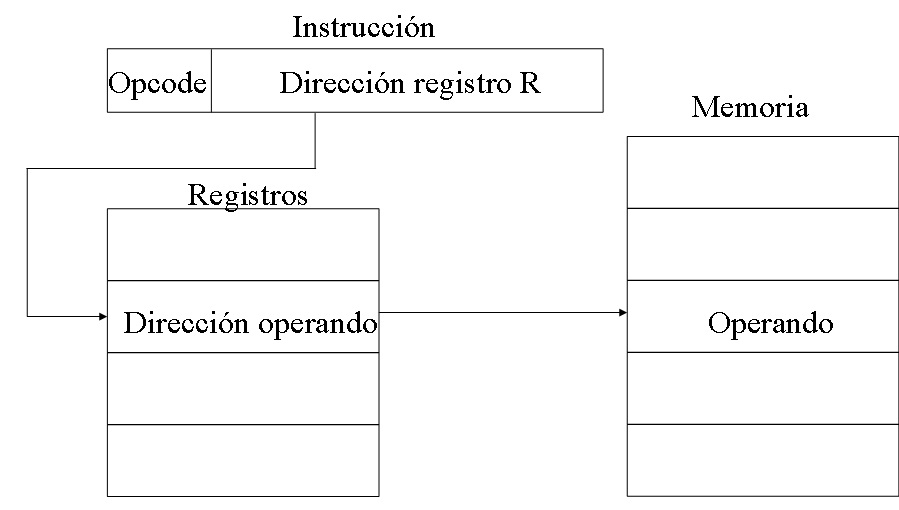
\includegraphics[scale=0.4]{imagenes/indirectoRegistro.jpg}
	\caption{Direccionamiento indirecto con registro}
	\end{figure}			
	\end{block}		 		
\end{frame}% enumerados


\begin{frame}
	\frametitle{Modos de direccionamiento}
	\begin{block}{Direccionamiento con desplazamiento} \justify
		\begin{equation}
			EA = A + (R)
		\end{equation}
		Donde $EA$ es la dirección que resulta al sumar los contenidos del registro $(R)$ y $A$.
	\end{block}		 		
\end{frame}

\begin{frame}
	\frametitle{Modos de direccionamiento}
	\begin{block}{Direccionamiento con desplazamiento} 
	\begin{figure}[H]
	\centering
	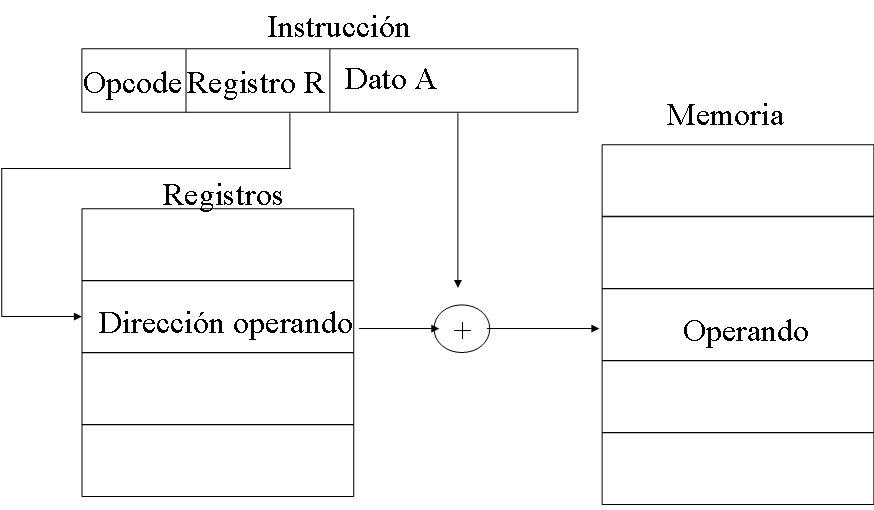
\includegraphics[scale=0.4]{imagenes/desplazamientoRegistro.jpg}
	\caption{Direccionamiento con desplazamiento con registro}
	\end{figure}			
	\end{block}		 		
\end{frame}


\section{Lenguaje ensamblador}

\subsection{Modelo procesador 8086/8088}

\begin{frame}
	\frametitle{Lenguaje ensamblador}
	\begin{figure}[H]
	\centering
	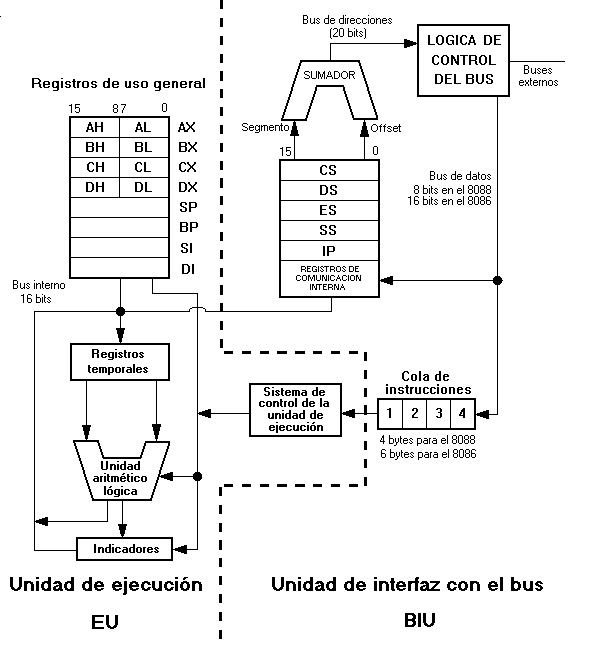
\includegraphics[scale=0.3]{imagenes/8088.png}
	\caption{Modelo procesador 8086/8088}
	\end{figure}			
\end{frame}



\begin{frame}
	\frametitle{Lenguaje ensamblador}
	\begin{block}{Registros}
		El 8086/88 dispone de 4 registros de datos, 4 registros de segmento, 5 registros de índice y 1
registro de estado.
	\end{block}		 		
\end{frame}

\begin{frame}
	\frametitle{Lenguaje ensamblador}
	\begin{block}{Registros de datos} \justify
			Los registros de datos son de 16 bits, aunque están divididos. lo que permite su acceso en 8 bits. Estos registros son de propósito general aunque todos tiene alguna función por defecto. 
			\begin{enumerate}
				\item \textbf{AX (acumulador)} se usa para almacenar el resultado de las operaciones, es al único registro con el que se puede hacer divisiones y multiplicaciones. Puede ser accedido en 8 bits como AH para la parte alta (HIGH) y AL (LOW) para la parte baja. 
				\item \textbf{BX (registro base)} almacena la dirección base para los accesos a memoria. También puede accederse como BH y BL, parte alta y baja respectivamente.
			\end{enumerate}
	\end{block}		 		
\end{frame}

\begin{frame}
	\frametitle{Lenguaje ensamblador}
	\begin{block}{Registros de datos} \justify
			Los registros de datos son de 16 bits, aunque están divididos. lo que permite su acceso en 8 bits. Estos registros son de propósito general aunque todos tiene alguna función por defecto. 
			\begin{enumerate}\setcounter{enumi}{2}
				\item \textbf{CX (contador)} actúa como contador en los bucles de repetición. CL (parte baja del registro) almacena el desplazamiento en las operaciones de desplazamiento y rotación de múltiples bits. 
				\item \textbf{DX (datos)} es usado para almacenar los datos de las operaciones. 
			\end{enumerate}
	\end{block}		 		
\end{frame}

\begin{frame}
	\frametitle{Lenguaje ensamblador}
	\begin{block}{Registros de segmento} \justify
		Los registros de segmento son de 16 bits y contienen el valor de segmento. 
		\begin{enumerate}
			\item \textbf{CS (segmento de código)} contiene el valor de segmento donde se encuentra el código. Actúa en conjunción con el registro IP (que veremos más adelante) para obtener la dirección de memoria que contiene la próxima instrucción.
			\item \textbf{DS (segmento de datos)}contiene el segmento donde están los datos
		\end{enumerate}
	\end{block}		 		
\end{frame}

\begin{frame}
	\frametitle{Lenguaje ensamblador}
	\begin{block}{Registros de segmento} \justify
		Los registros de segmento son de 16 bits y contienen el valor de
segmento. 
		\begin{enumerate}\setcounter{enumi}{2}
			\item \textbf{ES (segmento extra de datos)} es usado para acceder a otro segmento que contiene más datos. 
			\item \textbf{SS (segmento de pila)} contiene el valor del segmento donde está la pila. Se usa conjuntamente con el registro SP para obtener la dirección donde se encuentra el último valor almacenado en la pila por el procesador
		\end{enumerate}
	\end{block}		 		
\end{frame}

\begin{frame}
		\frametitle{Lenguaje ensamblador}
		\begin{block}{Registros de índice} \justify
Estos registros son usados como índices por algunas instrucciones. También pueden ser usados como operandos (excepto el registro IP).
			\begin{enumerate}\setcounter{enumi}{2}
				\item \textbf{DI (índice de destino)} almacena el desplazamiento del operando de destino en memoria en algunos tipos de operaciones (operaciones con operandos en memoria).
				\item \textbf{SP (índice de pila)} almacena el desplazamiento dentro del segmento de pila, y apunta al último elemento introducido en la pila. Se usa conjuntamente con el registro SS.
				\item \textbf{BP (índice de base)} se usa para almacenar desplazamiento en los distintos segmentos. Por defecto es el segmento de la pila 
		\end{enumerate}
	\end{block}		 		
\end{frame}


\begin{frame}
		\frametitle{Lenguaje ensamblador}
		\begin{block}{Registros de índice} \justify
Estos registros son usados como índices por algunas instrucciones. También pueden ser usados
como operandos (excepto el registro IP).
			\begin{enumerate}\setcounter{enumi}{2}
				\item \textbf{ES (segmento extra de datos)} es usado para acceder a otro segmento que contiene más datos. 
				\item \textbf{SS (segmento de pila)} contiene el valor del segmento donde está la pila. Se usa conjuntamente
con el registro SP para obtener la dirección donde se encuentra el último valor almacenado en la
pila por el procesador
			\end{enumerate}
	\end{block}		 		
\end{frame}

\begin{frame}
	\frametitle{Lenguaje ensamblador}
	\begin{block}{Registros de estado} \justify
El registro de estado contiene una serie de banderas que indican distintas situaciones en las que
se encuentra el procesador 
		\begin{figure}[H]
		\centering
		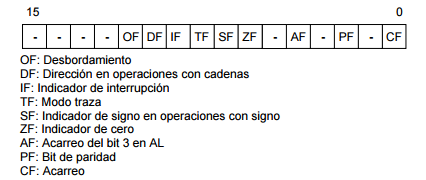
\includegraphics[scale=0.4]{imagenes/banderas.png}
		\caption{Estado del procesador}
		\end{figure}			
	\end{block}		 		
\end{frame}


\begin{frame}
	\frametitle{Lenguaje ensamblador}
	\begin{block}{Registros de estado} \justify
El registro de estado contiene una serie de banderas que indican distintas situaciones en las que
se encuentra el procesador 
	\begin{enumerate}
		\item OF (desbordamiento) es el principal indicador de error producido durante las operaciones con
signo. Vale 1 cuando:	
			\begin{itemize}
				\item La suma de dos números con igual signo o la resta de dos números con signo opuesto
producen un resultado que no se puede guardar (más de 16 bits).
				\item El bit más significativo (el signo) del operando ha cambiado durante una operación de desplazamiento aritmético.
				\item El resultado de una operación de división produce un cociente que no cabe en el registro de resultado
			\end{itemize} .
	\end{enumerate}	
	\end{block}			 		
\end{frame}

\begin{frame}
	\frametitle{Lenguaje ensamblador}
	\begin{block}{Registros de estado} \justify
El registro de estado contiene una serie de banderas que indican distintas situaciones en las que
se encuentra el procesador 
	\begin{enumerate}\setcounter{enumi}{1}
		\item \textbf{DF (dirección en operaciones con cadenas)} si es 1 el sentido de recorrido de la cadena es de izquierda a derecha, si es 0 irá en sentido contrario.
		\item \textbf{IF (indicador de interrupción)} cuando vale 1 permite al procesador reconocer interrupciones. Si se pone a 0 el procesador ignorará las solicitudes de interrupción.
		\item \textbf{TF (modo traza)} indica al procesador que la ejecución es paso a paso. Se usa en la fase de depuración.
		\item \textbf{SF (indicador de signo)} solo tiene sentido en las operaciones con signo. Vale 1 cuando en una de estas operaciones el signo del resultado es negativo.
	\end{enumerate}	
	\end{block}			 		
\end{frame}

\begin{frame}
	\frametitle{Lenguaje ensamblador}
	\begin{block}{Registros de estado} \justify
El registro de estado contiene una serie de banderas que indican distintas situaciones en las que se encuentra el procesador 
	\begin{enumerate}\setcounter{enumi}{6}
		\item \textbf{ZF (indicador de cero)} vale 1 cuando el resultado de una operación es cero.
		\item \textbf{AF (acarreo auxiliar)} vale 1 cuando se produce acarreo o acarreo negativo en el bit 3.
		\item \textbf{PF (paridad)} vale 1 si el resultado de la operación tiene como resultado un número con un número
par de bits a 1. Se usa principalmente en transmisión de datos.
		\item \textbf{CF (bit de acarreo)} vale 1 si se produce acarreo en una operación de suma, o acarreo negativo en una operación de resta. Contiene el bit que ha sido desplazado o rotado fuera de un registro o posición de memoria. Refleja el resultado de una comparación. 
	\end{enumerate}	
	\end{block}			 		
\end{frame}


\subsection{Generalidades}

\begin{frame}
		\frametitle{Lenguaje ensamblador}
		\begin{block}{Motivación}
		\begin{center}
			\large{¡Ha llegado la hora muchachos!\\Empieza lo bueno del curso}
			\begin{figure}[H]
				\centering
				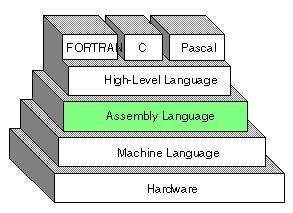
\includegraphics[scale=0.6]{imagenes/ensamblador.jpg}
				\caption{Lenguaje ensamblador}
			\end{figure}
		\end{center}
	\end{block}		 		
\end{frame}


\begin{frame}
		\frametitle{Lenguaje ensamblador}
		\begin{block}{Definiciones}
		\begin{center}
			\begin{enumerate}
				\item Las instrucciones en ensamblador se convierten directamente en lenguaje de máquina
				\item Tiene dos segmentos de memoria: programa y datos, recuerden el modelo de Von Neuman.
				\item El programa inicia en la posición de memoria 101
				\item Los datos inician en la posición de memoria 201
				\item En el curso vamos a utilizar ensamblador para el modelo de procesador 8086/8088. Este lo veremos la próxima clase.
			\end{enumerate}
		\end{center}
	\end{block}		 		
\end{frame}

\begin{frame}
		\frametitle{Lenguaje ensamblador}
		\begin{block}{Tipos de datos}
		\begin{center}
			\begin{enumerate}
				\item \textbf{Nibble:} 4 bits
				\item \textbf{Byte:} 8 bits
				\item \textbf{Word:} 16 bits
				\item \textbf{DWord:} 32 bits
			\end{enumerate}
		\end{center}
	\end{block}	
	\begin{block}{Representación datos}
	\begin{enumerate}
		\item Binario: $10101b$
		\item Hexadecimal: $6h$
		\item Decimal $6$
		\item Texto $'c'$ o $"casa"$
	\end{enumerate}
	\end{block}		 		
\end{frame}

\begin{frame}
	\frametitle{Lenguaje ensamblador}
	\begin{block}{Representación textos}
		\begin{itemize}
			\item Para el computador los textos son secuencias de números
			\item Por ejemplo 'c' es equivalente a tener $99$
			\item Esto es muy importante, ya que en ensamblador cuando se capturan los textos del teclado se captura su valor numérico, por ejemplo si presionamos 'c' en el teclado, se obtendrá $99$
			\item Existen dos extensiones de código ASCII, de 128 caracteres (simple) y 256 (extendido)
		\end{itemize}			
		
	\end{block}		 		
\end{frame}

\begin{frame}
	\frametitle{Lenguaje ensamblador}
	\begin{center}
		\begin{figure}[H]
			\centering
			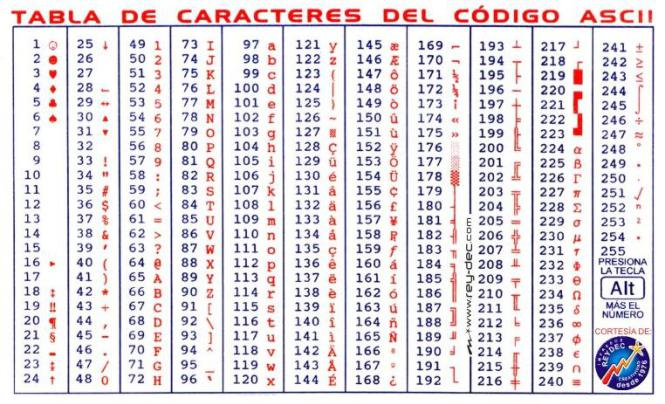
\includegraphics[scale=0.6]{imagenes/ASCII.jpg}
			\caption{Código ASCII}
		\end{figure}
	\end{center}
\end{frame}

\subsection{Direccionamiento en ensamblador}


\begin{frame}[fragile]
	\frametitle{Lenguaje ensamblador}
	\begin{block}{Direccionamiento de registro}
		Cuando ambos operadores son un registro
		\begin{lstlisting}
			MOV AX,BX ; Transfiere el contenido de BX a AX
		\end{lstlisting}
	\end{block}		 		
\end{frame}



\begin{frame}[fragile]
	\frametitle{Lenguaje ensamblador}
	\begin{block}{Direccionamiento inmediato}
		Cuando el operador origen es una constante
		\begin{lstlisting}
			MOV AX, 500; Carga en AX el valor 500
		\end{lstlisting}
	\end{block}		 		
\end{frame}


\begin{frame}[fragile]
	\frametitle{Lenguaje ensamblador}
	\begin{block}{Direccionamiento directo}
		Cuando el operando es una dirección de memoria
		\begin{lstlisting}
			MOV BX, [1000]; Almacena en BX el contenido de la dirección 1000 de memoria
			MOV AX, TABLA; Almacena en AX el contenido de la dirección en la constante TABLA
		\end{lstlisting}
		Luego se explicará como definir constantes
	\end{block}		 		
\end{frame}

\begin{frame}
	\frametitle{Lenguaje ensamblador}
	\begin{block}{Direccionamiento directo}
			\begin{figure}[H]
				\centering
				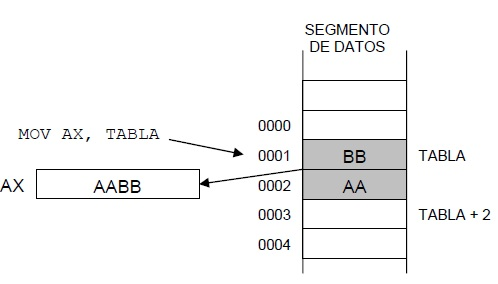
\includegraphics[scale=0.6]{imagenes/ensambladordirecto.jpg}
				\caption{Lenguaje ensamblador}
			\end{figure}
	\end{block}		 		
\end{frame}

\begin{frame}[fragile]
	\frametitle{Lenguaje ensamblador}
	\begin{block}{Direccionamiento indirecto}
		Cuando el operador está en memoria en una posición contenida por un registro
		\begin{lstlisting}
			MOV AX, [BX]; Almacena en AX el contenido de la dirección de memoria de BX
			MOV [BP], CX; Almacena en la dirección en memoria indicada por el contenido BP el dato de CX
		\end{lstlisting}
	\end{block}
\end{frame}
	
\begin{frame}
	\frametitle{Lenguaje ensamblador}
	\begin{block}{Direccionamiento directo}
			\begin{figure}[H]
				\centering
				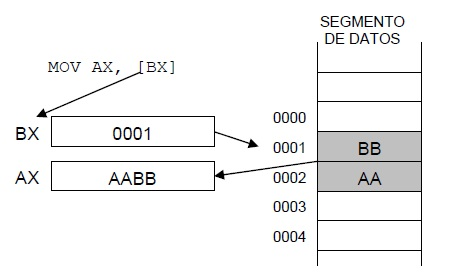
\includegraphics[scale=0.6]{imagenes/ensambladorindirecto.jpg}
				\caption{Lenguaje ensamblador}
			\end{figure}
	\end{block}		 		
\end{frame}


\begin{frame}[fragile]
	\frametitle{Lenguaje ensamblador}
	\begin{block}{Direccionamiento por registro base}
		Cuando el operando esta en memoria en una posición apuntada por un registro al que se le añade un determinado desplazamiento
		\begin{lstlisting}
			MOV AX, [BP] + 2; Almacena en AX el contenido de la dirección de memoria que se calcula al sumar 2 al contenido de BP
		\end{lstlisting}
	\end{block}
\end{frame}

\begin{frame}
	\frametitle{Lenguaje ensamblador}
	\begin{block}{Direccionamiento por registro base}
		\begin{figure}[H]
			\centering
			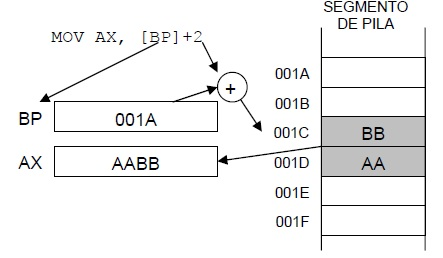
\includegraphics[scale=0.6]{imagenes/ensambladorbase.jpg}
			\caption{Lenguaje ensamblador}
		\end{figure}
	\end{block}		 		
\end{frame}


\begin{frame}[fragile]
	\frametitle{Lenguaje ensamblador}
	\begin{block}{Direccionamiento indexado}
		Cuando el operando es obtenido como la suma de un desplazamiento más el contenido de un registro
		\begin{lstlisting}
			MOV AX, TABLA[DI]; Almacena en AX el contenido de la dirección de memoria que se calcula al sumar TABLA al contenido de DI
		\end{lstlisting}
	\end{block}
\end{frame}

\begin{frame}
	\frametitle{Lenguaje ensamblador}
	\begin{block}{Direccionamiento indexado}
		\begin{figure}[H]
			\centering
			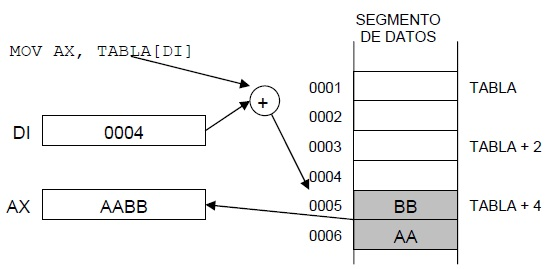
\includegraphics[scale=0.6]{imagenes/ensamabladorindexado.jpg}
			\caption{Lenguaje ensamblador}
		\end{figure}
	\end{block}		 		
\end{frame}

\begin{frame}[fragile]
	\frametitle{Lenguaje ensamblador}
	\begin{block}{Direccionamiento indexado respecto a una base}
		Cuando el operando es obtenido como la suma de un desplazamiento más el contenido de un registro
		\begin{lstlisting}
			MOV AX, TABLA[BX][DI]; Almacena en AX el contenido de la dirección de memoria que se calcula al sumar TABLA al contenido de DI más el contenido del registro BX
		\end{lstlisting}
	\end{block}
\end{frame}

\subsection{Juegos de instrucciones}

\begin{frame}
	\frametitle{Lenguaje ensamblador}
	\begin{block}{Juegos de instrucciones}
		Las instrucciones del 8086/8088 se dividen en:
		\begin{enumerate}
			\item Instrucciones de transferencia de datos
			\item Instrucciones aritméticas
			\item Instrucciones lógicas
			\item Instrucciones de desplazamiento
			\item Instrucciones E/S
			\item Instrucciones de control de flujo
		\end{enumerate}
	\end{block}
\end{frame}

\begin{frame}
	\frametitle{Lenguaje ensamblador}
	\begin{block}{Instrucciones de transferencia de datos}
		\begin{enumerate}
			\item \textbf{MOV:} Realiza la transferencia de datos de origen a destino
			\item \textbf{XCHG:} Realiza el intercambio entre los valores de los operandos
			\item \textbf{LEA:} Carga en un registro la dirección efectiva especificada
			\item \textbf{PUSH} \textbf{POP}: Realizan las operaciones de apilado y desapilado en la pila del procesador
		\end{enumerate}
	\end{block}
\end{frame}

\begin{frame}
	\frametitle{Lenguaje ensamblador}
	\begin{block}{Instrucciones aritméticas}
		\begin{enumerate}
			\item \textbf{ADD:} Realiza la suma
			\item \textbf{SUB:} Realiza la resta
			\item \textbf{NEG:} Realiza la negación de un operando
			\item \textbf{MUL:} Realiza la multiplicación, para 8 bits guarda el resultado en AX, para 16 bits, guarda en la combinación DX:AX
			\item \textbf{DIV:} Realiza la división sin signo, para 8 bits guarda el cociente en AL y el resto en AH, para 16 bits guarda el cociente en AX y el resto en DX
		\end{enumerate}
	\end{block}
\end{frame}

\begin{frame}
	\frametitle{Lenguaje ensamblador}
	\begin{block}{Instrucciones lógicas}
		\begin{enumerate}
			\item \textbf{OR, XOR AND:} Realiza operaciones lógicas
			\item \textbf{NOT:} Operación lógica de complemento
		\end{enumerate}
	\end{block}
\end{frame}

\begin{frame}
	\frametitle{Lenguaje ensamblador}
	\begin{block}{Instrucciones de comparación}
		\begin{enumerate}
			\item \textbf{CMP:} Realiza la resta de dos operandos, pero no afecta a ninguno. Esta afecta a las banderas del procesador, lo que se verá más adelante.
		\end{enumerate}
	\end{block}
\end{frame}

\begin{frame}
	\frametitle{Lenguaje ensamblador}
	\begin{block}{Instrucciones de desplazamiento}
		\begin{enumerate}
			\item \textbf{SAL/SHL:} Introduce un 0 al final del registro y desplaza hacia la izquierda el resto de bits. El primer bit es almacenado en el registro de estado.
			\item \textbf{SAR:} Desplazamiento de la derecha
		\end{enumerate}
	\end{block}
\end{frame}

\begin{frame}
	\frametitle{Lenguaje ensamblador}
	\begin{block}{Instrucciones de E/S}
	Se utilizan para comunicación con periféricos
		\begin{enumerate}
			\item \textbf{IN:} Leer un puerto.
			\item \textbf{OUT:} Escribir en un puerto
		\end{enumerate}
	\end{block}
\end{frame}

\begin{frame}
	\frametitle{Lenguaje ensamblador}
	\begin{block}{Instrucciones de control de flujo}
	Se utilizan después es ejecutar el comando \textbf{CMP}
		\begin{enumerate}
			\item \textbf{JMP:} Permite saltar a otras partes del código. Esta no requiere la ejecución de CMP.
			\item \textbf{JE/JZ:} Indica que los dos operadores son iguales
			\item \textbf{JA} Si el primer operador es mayor que el segundo
			\item \textbf{JB} Si el primer operador es menor que el segundo
			\item \textbf{JNZ}: Si los dos operadores son diferentes
		\end{enumerate}
	\end{block}
\end{frame}

\begin{frame}
	\frametitle{Lenguaje ensamblador}
	\begin{block}{Instrucciones de control de flujo}
			\begin{enumerate}
			\item \textbf{LOOP:} Se utiliza para realizar bucles repetitivos, se utiliza el registro \textbf{CX} para indicar el número de veces que se realiza el ciclo, este debe apuntar a una estructura
		\end{enumerate}
	\end{block}
\end{frame}

\subsection{Etiquetas, comentarios y directivas}

\begin{frame}[fragile]
	\frametitle{Lenguaje ensamblador}
	\begin{block}{Etiquetas, comentarios y directivas}
			\begin{enumerate}
			\item Una etiqueta da el nombre a una instrucción y esto permite hacer referencia a ella
			\begin{lstlisting}
				INICIO: MOV CX, DI ; inicia el contador
			\end{lstlisting}
			\item Los comentarios son antecedidos por ;
		\end{enumerate}
	\end{block}
\end{frame}

\begin{frame}
	\frametitle{Lenguaje ensamblador}
	\begin{block}{Etiquetas, comentarios y directivas}
		Una directiva sirve para definir segmentos
			\begin{enumerate}
				\item \textbf{.MODEL} Se utilizan en las directivas simplificadas: 
				\begin{itemize}
					\item \textbf{TINY} Para programas solo segmentos datos y codigo
					\item \textbf{SMALL} Para programas son solo segemento de datos (64K memoria) y otro de código (64k)
					\item \textbf{LARGE} Para programas segmento de datos y código (1MB para cada uno)
					\item \textbf{MEDIUM:} Varios segmentos de código y varios de datos
					\item \textbf{COMPACT:} 1 segmento de código y varos de datos
				\end{itemize}
				\item \textbf{.STACK n} Define el tamaño de la pila, por defecto 1KB
				\item \textbf{.DATA} Abre segmento de datos
				\item \textbf{.CODE} Abre segmento de código
			\end{enumerate}
	\end{block}
\end{frame}

\begin{frame}[fragile]
	\frametitle{Lenguaje ensamblador}
	\begin{block}{Etiquetas, comentarios y directivas}
		Una directiva sirve para definir segmentos
		\begin{enumerate}
			\item \textbf{EQU:} Define una directiva
				\begin{lstlisting}
				CONSTANTE EQU 1020; Constante toma el valor 1023
				\end{lstlisting}				
			\item DB, DW y DD se utilizan para definir el tamaño de las variables en memoria, DB byte, DW tamaño word y DD tamaño DWORD
			\begin{lstlisting}
				MENSAJE DB 'Este es un mensaje' ; Reserva una constante de tamaño byte para el mensaje
				PESO DW ? ;Reserva una variable tamaño DWord, pero no tiene valor debido a ?
			\end{lstlisting}	
		\end{enumerate}
	\end{block}
\end{frame}

\begin{frame}[fragile]
	\frametitle{Lenguaje ensamblador}
	\begin{center}	
	\begin{lstlisting}
		.MODEL SMALL
		.STACK 100H
		.DATA
		    max EQU 100
		    cad DB max DUP ?
		    dac DB max DUP ?
		.CODE
		    MOV AX, @DATA
		    MOV DS, AX
		 END
	\end{lstlisting}
	\end{center}				
\end{frame}



\begin{frame}
	\frametitle{Preguntas}
	\vfill
	\begin{center}
	¿Preguntas?\\
	\vfill
	Siguiente clase: \\
	Repertorio de Instrucciones: \\
	Estructura y funcionamiento del procesador
	\end{center}
\end{frame}


\end{document}